\chapter{Results}\label{sec:results}
We now describe the results of testing the ILP systems. Due to restraints on computational power we tested the performance of the each ILP on 8 full game play outs. 15 minutes were given for each system to generate a hypothesis. We trained the systems on random gameplay, gameplay generated by the Sancho system and then a mixture of both. The generated hypotheses were tested on both Sancho generated and random gameplay examples. We used a selection of 35 games from the IGGP dataset\cite{Cropper/IGGP}. The full dataset was not used due to issues of compatibility with the Sancho system.

In the IGGP paper\cite{Cropper/IGGP} the IGGP task was defined across four predicates for each game: \textit{goal}, \textit{next}, \textit{terminal} and \textit{legal}. After testing the systems on all four predicates it was found that the terminal predicates did not give an accurate picture into the ability to learn of each system. Each game had a maximum number of moves, these varied from game to game. Generally the randomly generated game traces did not complete the game before the move limit was reached. Since the terminal predicate is true on the last game state in each game and the game state includes a move counter this allowed the systems to simply learn the correlation between the maximum move and the terminal predicate. They would learn the program: \verb|terminal :- true_step(MAX)| where \verb|MAX| is the maximum number of moves for the game. This means that when a game is played randomly and the max move count is always hit the predicate is perfectly solved, however if when Sancho plays then game it solves it before the maximum moves is hit it is less likely to induce a correct rule. For this reason the \textit{terminal} predicate was left out of the aggregated scores.


Q1 Does varying the quality of game traces influence the ability for learners to solve the IGGP problems? Specifically, does the quality of game play affect predictive accuracy?
Q2 Does varying the amount of game traces influence the ability for learners to solve the IGGP problems? Specifically, does the quality of game play affect predictive accuracy?
Q3 Can we improve the performance of a learner by mixing the quality of traces?

\section{Evaluation metrics}
To evaluate the performance of the ILP systems on the training dataset we use two metrics: balanced accuracy and perfectly solved.

\textbf{Balanced accuracy} In the datasets used for testing the ILP systems the vast majority of examples are negative. Balanced accuracy takes this into account when evaluating approaches. The system to be tested is the generated logical hypothesis $H$ which, along with the background knowledge $B$ for the relevant game. The test data is the set of combined positive and negative testing examples $E^+ \cup E^-$. We define the number of positive examples $p = |E^+|$, the number of negative examples $n = |E^-|$, the number of correctly predicted positives as $tp = |\{e\in E^+|B\cup H \models e\}|$ and the number of correctly predicted negatives as $tn = |\{e\in E^-|B\cup H \not\models e\}|$. The balanced accuracy is subsequently defined as $ba = 100 \cdot (tp/p + tn/n)/2$.

\textbf{Perfectly solved} This metric considers the number of predicates for which the ILP system correctly classified all examples. It is equivalent to the number of games with a balanced accuracy score of 100. This metric is important since for all predicates there exists an exact solution (the rules that were used to generate the examples). A system that has correctly predicated 99\% of the results is no where near as useful as one that predicts 100\%.

\section{Answering research questions}
To answer the research questions one and three we train the three ILP systems on random, Sancho generated game traces as well as a mixture of the two. We compare the average balanced accuracy and the number of perfectly solved games of the different systems trained on the range of domains. 

To answer question two we train the systems on the mixed traces with varying size of data to see how it affects the test results. We train on the mixed traces since this gave the best results in the first set of experiments.
\section{Results summary}
We present the conglomerated results in two forms. As a table and as a bar graph. The full results for each game and predicate learned are too lengthy to include in this paper. They can however be found in the code repository\footnote{https://github.com/Aflynn50/GPP-3rd-year-project} as well as by rerunning the experiment. 

We found that overall the systems trained on the mixed data did better than the systems trained on random data. However the difference in score was not particularly pronounced.

Aleph was limited by the maximum size of the program to be learned. This affected its performance on the larger number of traces. Aleph often did well at learning the \textit{goal} and \textit{next} predicates however was generally scored poorly on the more complex \textit{legal} predicate. The system did not do significantly better on optimal or random. It performed well when trained and tested on the Sancho traces. 

The Metagol system was ineffective across all sets of data. It sometime managed to learn part of the \textit{next} predicate for some games but never managed \textit{legal} or \textit{goal} predicates.

The programs that were learned by the Aleph system almost always consisted of a conjunction of the examples in the training set. This method was only effective 




When increasing the number of traces it was observed that the there was a large jump in effectiveness of ILASP between 8 and 16 traces but between 16 and 24 traces the aggregated results were identical suggesting the new extra game traces had no benefit to the ILP systems. The number of games the ILASP perfectly solved also jumped by a huge amount, from 7-8 to 76 suggesting that this system in particular benefited a lot from the extra data.

Balanced accuracy

\begin{table}[]
	\begin{tabular}{|c|c|c|c|c|c|c|}
		\hline
		\multicolumn{7}{|c|}{Balanced Accuracy}                                                                           \\ \hline
		\multirow{2}{*}{Systems} & \multicolumn{2}{c|}{Random} & \multicolumn{2}{c|}{Sancho} & \multicolumn{2}{c|}{Mixed} \\ \cline{2-7} 
		& Random       & Sancho       & Random       & Sancho       & Random       & Sancho      \\ \hline
		Metagol                  & 51           & 51           & 51           & 51           & 51           & 51          \\ \hline
		Aleph                    & 66           & 65           & 65           & 72           & 80           & 66          \\ \hline
		ILASP                    & 72           & 72           & 71           & 72           & 73           & 73          \\ \hline
	\end{tabular}
\end{table}


\begin{table}[]
	\begin{tabular}{|c|c|c|c|c|c|c|}
		\hline
		\multicolumn{7}{|c|}{Perfectly Solved}                                                                            \\ \hline
		\multirow{2}{*}{Systems} & \multicolumn{2}{c|}{Random} & \multicolumn{2}{c|}{Sancho} & \multicolumn{2}{c|}{Mixed} \\ \cline{2-7} 
		& Random       & Sancho       & Random       & Sancho       & Random       & Sancho      \\ \hline
		Metagol                  & 0            & 0            & 0            & 0            & 0            & 0           \\ \hline
		Aleph                    & 1            & 0            & 0            & 4            & 7            & 0           \\ \hline
		ILASP                    & 7            & 8            & 5            & 10           & 7            & 8           \\ \hline
	\end{tabular}
\end{table}

\begin{table}[]
	\begin{tabular}{|c|c|c|c|c|c|c|}
		\hline
		\multicolumn{7}{|c|}{Balenced Accuracy}                                                                                       \\ \hline
		\multirow{2}{*}{Systems} & \multicolumn{2}{c|}{Mixed - 8} & \multicolumn{2}{c|}{Mixed - 16} & \multicolumn{2}{c|}{Mixed - 24} \\ \cline{2-7} 
		& Random         & Sancho        & Random         & Sancho         & Random         & Sancho         \\ \hline
		Metagol                  & 51             & 51            & 51             & 51             & 51             & 51             \\ \hline
		Aleph                    & 80             & 66            & 67             & 65             & 67             & 65             \\ \hline
		ILASP                    & 73             & 73            & 85             & 85             & 85             & 85             \\ \hline
	\end{tabular}
\end{table}

\begin{table}[]
	\begin{tabular}{|c|c|c|c|c|c|c|}
		\hline
		\multicolumn{7}{|c|}{Perfectly Solved}                                                                                        \\ \hline
		\multirow{2}{*}{Systems} & \multicolumn{2}{c|}{Mixed - 8} & \multicolumn{2}{c|}{Mixed - 16} & \multicolumn{2}{c|}{Mixed - 24} \\ \cline{2-7} 
		& Random         & Sancho        & Random         & Sancho         & Random         & Sancho         \\ \hline
		Metagol                  & 0              & 0             & 0              & 0              & 0              & 0              \\ \hline
		Aleph                    & 7              & 0             & 0              & 0              & 0              & 0              \\ \hline
		ILASP                    & 7              & 8             & 76             & 76             & 76             & 76             \\ \hline
	\end{tabular}
\end{table}

\section{Varying quality training data}

\subsubsection{Random training}
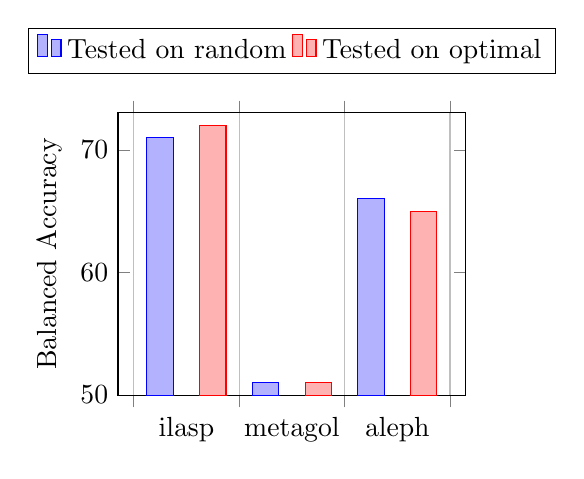
\begin{tikzpicture}
\begin{axis}[
	ylabel=Balanced Accuracy,
	width=6cm,
	enlargelimits=0.05,
	legend style={at={(0.5,1.3)},
	anchor=north,
	legend columns=-1},
	ybar interval=0.5,
	symbolic x coords={ilasp,metagol,aleph, poog}
]
\addplot 
	coordinates {(ilasp,71) (metagol,51) (aleph,66) (poog, 65)};
\addplot 
	coordinates {(ilasp,72) (metagol,51) (aleph,65) (poog,65)};
\legend{Tested on random,Tested on optimal}
\end{axis}
\end{tikzpicture}
~
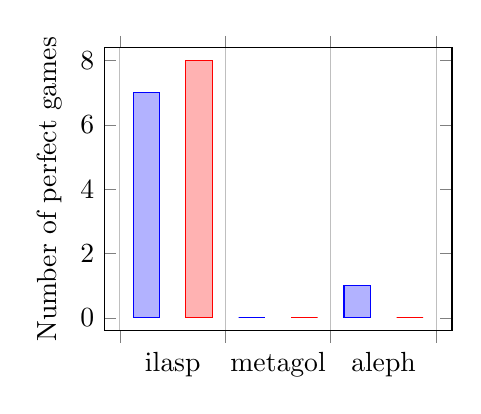
\begin{tikzpicture}
\begin{axis}[
	width=6cm, 
	ylabel=Number of perfect games,
	enlargelimits=0.05,
	ybar interval=0.5,
	symbolic x coords={ilasp,metagol,aleph, poog}
]
\addplot 
	coordinates {(ilasp,7) (metagol,0) (aleph,1) (poog, 0)};
\addplot 
	coordinates {(ilasp,8) (metagol,0) (aleph,0) (poog,0)};
\end{axis}
\end{tikzpicture}
\subsubsection{Optimal training}
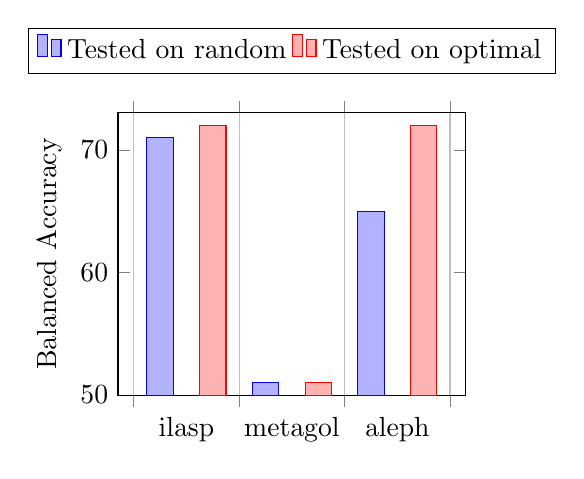
\begin{tikzpicture}
\begin{axis}[
ylabel=Balanced Accuracy,
width=6cm,
enlargelimits=0.05,
legend style={at={(0.5,1.3)},
	anchor=north,
	legend columns=-1},
ybar interval=0.5,
symbolic x coords={ilasp,metagol,aleph, poog}
]
\addplot 
coordinates {(ilasp,71) (metagol,51) (aleph,65) (poog, 65)};
\addplot 
coordinates {(ilasp,72) (metagol,51) (aleph,72) (poog,65)};
\legend{Tested on random,Tested on optimal}
\end{axis}
\end{tikzpicture}
~
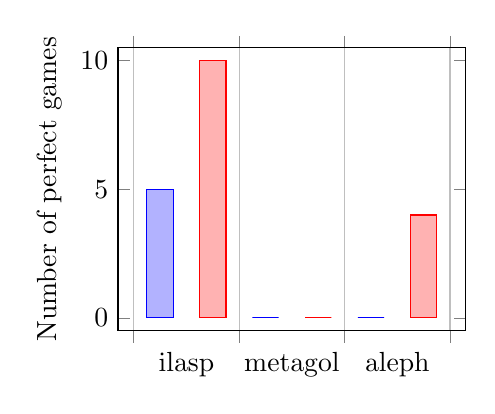
\begin{tikzpicture}
\begin{axis}[
width=6cm, 
ylabel=Number of perfect games,
enlargelimits=0.05,
ybar interval=0.5,
symbolic x coords={ilasp,metagol,aleph, poog}
]
\addplot 
coordinates {(ilasp,5) (metagol,0) (aleph,0) (poog, 0)};
\addplot 
coordinates {(ilasp,10) (metagol,0) (aleph,4) (poog,0)};
\end{axis}
\end{tikzpicture}
\subsubsection{Mixed training}
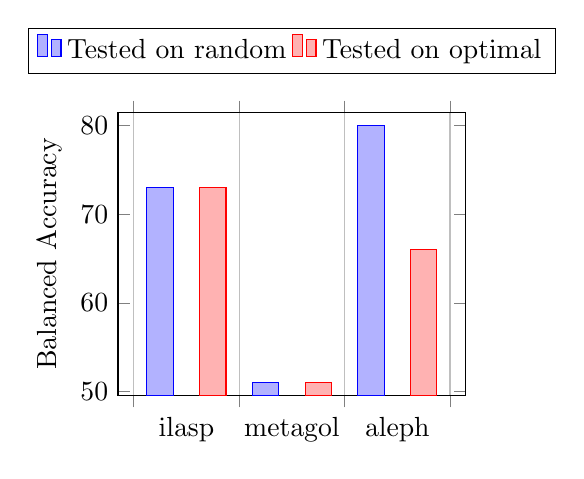
\begin{tikzpicture}
\begin{axis}[
ylabel=Balanced Accuracy,
width=6cm,
enlargelimits=0.05,
legend style={at={(0.5,1.3)},
	anchor=north,
	legend columns=-1},
ybar interval=0.5,
symbolic x coords={ilasp,metagol,aleph, poog}
]
\addplot 
coordinates {(ilasp,73) (metagol,51) (aleph,80) (poog,70)};
\addplot 
coordinates {(ilasp,73) (metagol,51) (aleph,66) (poog,70)};
\legend{Tested on random,Tested on optimal}
\end{axis}
\end{tikzpicture}
~
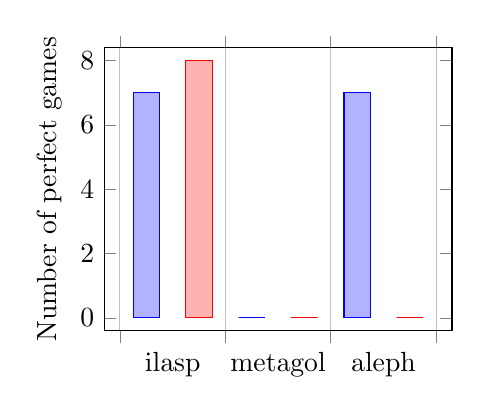
\begin{tikzpicture}
\begin{axis}[
width=6cm, 
ylabel=Number of perfect games,
enlargelimits=0.05,
ybar interval=0.5,
symbolic x coords={ilasp,metagol,aleph, poog}
]
\addplot 
coordinates {(ilasp,7) (metagol,0) (aleph,7) (poog, 0)};
\addplot 
coordinates {(ilasp,8) (metagol,0) (aleph,0) (poog,0)};
\end{axis}
\end{tikzpicture}

\subsubsection{Mixed training with 16 traces}
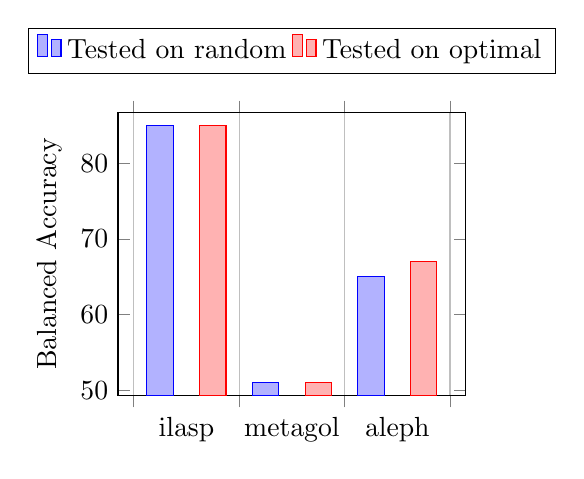
\begin{tikzpicture}
\begin{axis}[
ylabel=Balanced Accuracy,
width=6cm,
enlargelimits=0.05,
legend style={at={(0.5,1.3)},
	anchor=north,
	legend columns=-1},
ybar interval=0.5,
symbolic x coords={ilasp,metagol,aleph, poog}
]
\addplot 
coordinates {(ilasp,85) (metagol,51) (aleph,65) (poog,70)};
\addplot 
coordinates {(ilasp,85) (metagol,51) (aleph,67) (poog,70)};
\legend{Tested on random,Tested on optimal}
\end{axis}
\end{tikzpicture}
~
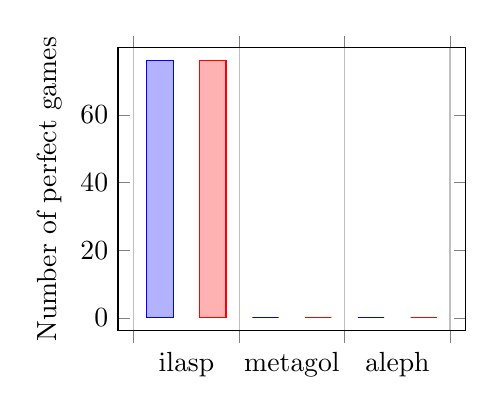
\begin{tikzpicture}
\begin{axis}[
width=6cm, 
ylabel=Number of perfect games,
enlargelimits=0.05,
ybar interval=0.5,
symbolic x coords={ilasp,metagol,aleph, poog}
]
\addplot 
coordinates {(ilasp,76) (metagol,0) (aleph,0) (poog, 0)};
\addplot 
coordinates {(ilasp,76) (metagol,0) (aleph,0) (poog,0)};
\end{axis}
\end{tikzpicture}

\subsubsection{Mixed training with 24 traces}
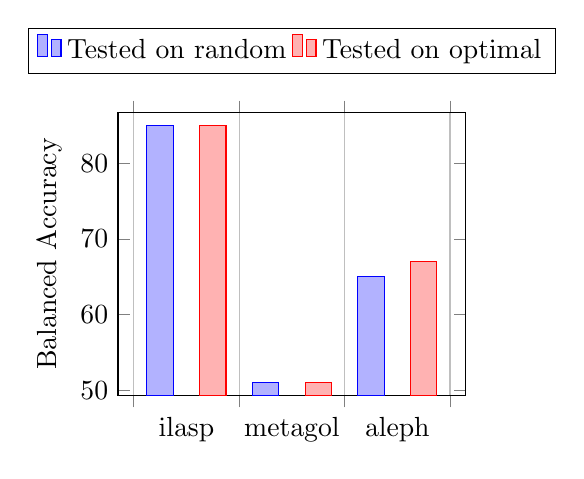
\begin{tikzpicture}
\begin{axis}[
ylabel=Balanced Accuracy,
width=6cm,
enlargelimits=0.05,
legend style={at={(0.5,1.3)},
	anchor=north,
	legend columns=-1},
ybar interval=0.5,
symbolic x coords={ilasp,metagol,aleph, poog}
]
\addplot 
coordinates {(ilasp,85) (metagol,51) (aleph,65) (poog,70)};
\addplot 
coordinates {(ilasp,85) (metagol,51) (aleph,67) (poog,70)};
\legend{Tested on random,Tested on optimal}
\end{axis}
\end{tikzpicture}
~
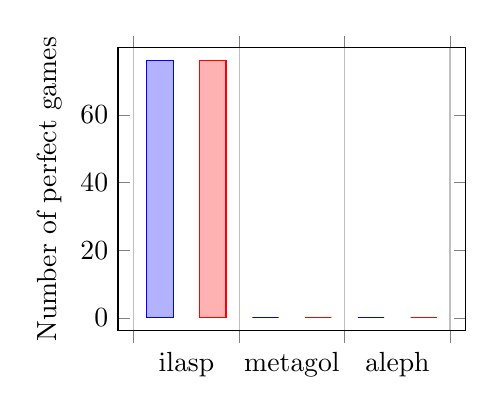
\begin{tikzpicture}
\begin{axis}[
width=6cm, 
ylabel=Number of perfect games,
enlargelimits=0.05,
ybar interval=0.5,
symbolic x coords={ilasp,metagol,aleph, poog}
]
\addplot 
coordinates {(ilasp,76) (metagol,0) (aleph,0) (poog, 0)};
\addplot 
coordinates {(ilasp,76) (metagol,0) (aleph,0) (poog,0)};
\end{axis}
\end{tikzpicture}

